\documentclass[conference]{IEEEtran}

\usepackage{amsmath}
\usepackage{amssymb}
\usepackage{graphicx}
\usepackage{xcolor}
\usepackage{tikz}
\usetikzlibrary{positioning,arrows.meta,decorations.pathreplacing}
% \usepackage[nocompress]{cite}
\usepackage[numbers,sort]{natbib}
\usepackage[margin=1in]{geometry}
\usepackage{parskip}

\title{Identifying $\epsilon$-Cohesive Cores on a Bipartite Graph}

\author{
\IEEEauthorblockN{Kiyaan Pillai}
}

\begin{document}

\maketitle

\section{Introduction}
\subsection{Bipartite Graphs and Bicliques}

\begin{itemize}
\item Do I explain the concepts well enough so a nonexpert audience can understand?
\item Credibility analysis
\end{itemize}


\begin{figure}[!t]
    \centering
    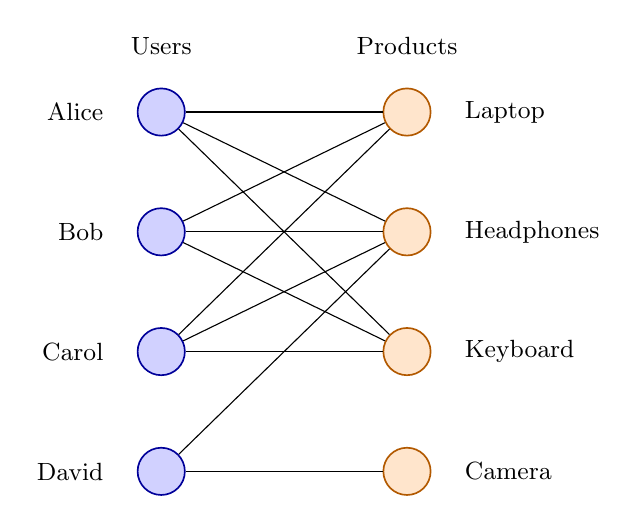
\begin{tikzpicture}[
        vertex/.style={
            circle,
            draw,
            minimum size=6mm,
            inner sep=0pt,
            line width=0.6pt
        },
        leftvertex/.style={
            vertex,
            fill=blue!18,
            draw=blue!60!black
        },
        rightvertex/.style={
            vertex,
            fill=orange!20,
            draw=orange!70!black
        },
        node distance=9mm and 25mm
    ]

        % Users
        \node[leftvertex] (u1) {};
        \node[leftvertex, below=of u1] (u2) {};
        \node[leftvertex, below=of u2] (u3) {};
        \node[leftvertex, below=of u3] (u4) {};

        % User labels
        \node[left=3mm of u1] {\small Alice};
        \node[left=3mm of u2] {\small Bob};
        \node[left=3mm of u3] {\small Carol};
        \node[left=3mm of u4] {\small David};

        % Products
        \node[rightvertex, right=of u1] (p1) {};
        \node[rightvertex, below=of p1] (p2) {};
        \node[rightvertex, below=of p2] (p3) {};
        \node[rightvertex, below=of p3] (p4) {};

        % Product labels
        \node[right=3mm of p1] {\small Laptop};
        \node[right=3mm of p2] {\small Headphones};
        \node[right=3mm of p3] {\small Keyboard};
        \node[right=3mm of p4] {\small Camera};

        % Edges forming a 3x3 biclique
        \draw (u1) -- (p1);
        \draw (u1) -- (p2);
        \draw (u1) -- (p3);

        \draw (u2) -- (p1);
        \draw (u2) -- (p2);
        \draw (u2) -- (p3);

        \draw (u3) -- (p1);
        \draw (u3) -- (p2);
        \draw (u3) -- (p3);

        % Additional edges outside the biclique
        \draw (u4) -- (p2);
        \draw (u4) -- (p4);

        % Part labels
        \node[above=3mm of u1] {\small Users};
        \node[above=3mm of p1] {\small Products};

    \end{tikzpicture}
    \caption{A bipartite user-product graph. Alice, Bob, and Carol each purchased the same three products, forming a $3\times3$ biclique, while David has a different set of purchases.}
    \label{fig:bipartite-example}
\end{figure}


Data can often be modeled on a graph of nodes and edges. The nodes represent distinct entities, and the edges represent interactions between those entities. For instance, Amazon may have a graph where the nodes represent items, and the edges connect two items that are often bought together. A bipartite graph is a type of graph where edges only exist between two sets of vertices that do not connect to each other. Many real-world datasets are naturally bipartite. For example, Amazon users can be linked to items they bought, but users are not linked to users and items are not linked to each other. In each case, the edges only run between two distinct kinds of entities \cite{zhang2025density}. In these graphs, dense clusters of vertices that are extremely connected often correspond to meaningful communities. For example, if a group of Amazon users all buy many of the same items, those users might have the same shopping preferences. A cluster of vertices is called a subgraph, and a dense subgraph like the Amazon example where all left-side vertices are connected to all right-side vertices is called a biclique. Identifying large bicliques can recover meaningful communities of users that have similar interests \cite{lehmann2008biclique, alzahrani2019finding}.

\begin{figure}[!t]
    \centering
    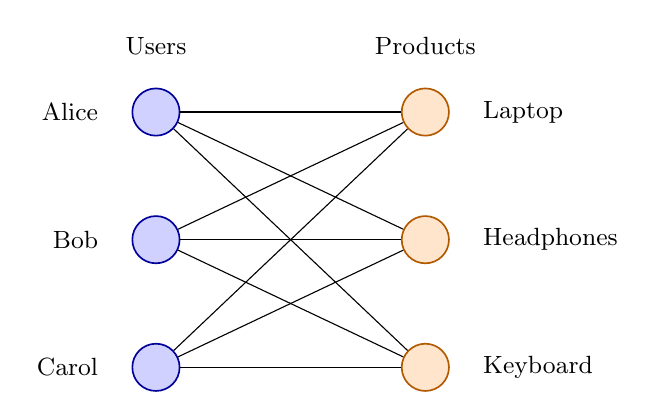
\begin{tikzpicture}[
        vertex/.style={
            circle,
            draw,
            minimum size=6mm,
            inner sep=0pt,
            line width=0.6pt
        },
        leftvertex/.style={
            vertex,
            fill=blue!18,
            draw=blue!60!black
        },
        rightvertex/.style={
            vertex,
            fill=orange!20,
            draw=orange!70!black
        },
        node distance=10mm and 28mm
    ]

        % Users
        \node[leftvertex] (u1) {};
        \node[leftvertex, below=of u1] (u2) {};
        \node[leftvertex, below=of u2] (u3) {};

        \node[left=3mm of u1] {\small Alice};
        \node[left=3mm of u2] {\small Bob};
        \node[left=3mm of u3] {\small Carol};

        % Products
        \node[rightvertex, right=of u1] (p1) {};
        \node[rightvertex, below=of p1] (p2) {};
        \node[rightvertex, below=of p2] (p3) {};

        \node[right=3mm of p1] {\small Laptop};
        \node[right=3mm of p2] {\small Headphones};
        \node[right=3mm of p3] {\small Keyboard};

        % Complete 3x3 biclique
        \draw (u1) -- (p1);
        \draw (u1) -- (p2);
        \draw (u1) -- (p3);

        \draw (u2) -- (p1);
        \draw (u2) -- (p2);
        \draw (u2) -- (p3);

        \draw (u3) -- (p1);
        \draw (u3) -- (p2);
        \draw (u3) -- (p3);

        % Part labels
        \node[above=3mm of u1] {\small Users};
        \node[above=3mm of p1] {\small Products};

    \end{tikzpicture}
    \caption{The $3\times3$ biclique contained within Figure~\ref{fig:bipartite-example}. Every user is connected to every product in the biclique.}
    \label{fig:biclique-example}
\end{figure}


Dense subgraphs are used for practical tasks. Hooi et al. \cite{hooi2017graph} designed FRAUDAR to detect coordinated fraud, in which many accounts purchase the same products to inflate each other's ratings, by detecting large bicliques. Zhang et al. \cite{zhang2025cohesive} apply a specialized biclique model to user-item graphs for recommendation and group discovery. Their work suggests that dense graph structures can be used for recommendation systems, and this is the use case on which we test our model.

\subsection{Biclique Formulations}

Because a biclique requires every vertex on one side of a network to connect to every vertex on the other, even one missing connection can cause an otherwise meaningful group to be overlooked. Walsh et al. \cite{walsh2016discovering} identify this strict requirement as a major source of false negatives in biological data, where meaningful relationships may exist despite missing connections. Yan et al. \cite{yan2005identifying} found that phylogenetic datasets with some missing connections could reveal evolutionary relationships nearly as accurately as complete datasets. Similarly, Zhang et al. \cite{zhang2025density} found that standard bicliques were too restrictive for email, movie, and club recommendation data, suggesting that useful groups can exist even when some connections are missing.

Biclique variations exist to overcome this strictness. These variations try to find large bipartite subgraphs that are almost entirely connected, even if not exactly. Sim et al. \cite{sim2009mining} introduced the quasi-biclique, which allows up to a certain percentage of edges to be missing, and it was later applied in bioinformatics settings and recommendation systems \cite{sim2009mining, li2008quasi, maulik2012mining, zhang2025density}. However, Li et al. \cite{li2008quasi} found that large quasi-bicliques often recovered completely different communities than exact bicliques. Yu et al. \cite{yu2021} introduced the $k$-biplex, which seeks large subgraphs where every vertex has at least $k$ connections to the other side. Zhou et al. \cite{zhou2025} generalized the $k$-biplex to the $(k, \ell)$-biplex, which is more restrictive and limits the number of missing edges per vertex. Cui et al. \cite{cui2025efficient} and Wang et al. \cite{wang2025defective} independently introduced the $k$-defective biclique, which finds bicliques with up to $k$ missing edges and sets a minimum vertex count $\theta$ for each side. Kim et al. \cite{kim2026} proposed the flexi-clique for non-bipartite graphs, in which each vertex must be connected to at least $|H|^\tau$ other vertices, where $|H|$ is the number of vertices in the subgraph and $\tau$ is a parameter controlling the required connectivity. Although originally developed for non-bipartite graphs, this approach could also be adapted to bipartite graphs.

\subsection{Limitations of Edge Relaxations}

Most biclique variations propose an allowed number of missing edges, but all of them require exact connections. This can impose unnecessary restrictions on the recovered structure. Two users who each bought different items from the same narrow category share no edges in common, yet a recommender system would reasonably treat them as similar.

Subgraphs that seek nodes similar to each other under a given similarity metric have been studied previously. Zhang et al. \cite{zhang2016core} defined the $(k, r)$-core, which requires each vertex to have at least $k$ neighbors in the subgraph and every pair of vertices to have similarity of at least $r$ given a similarity function. Zhu et al. \cite{zhu2017} and Li and Zlatanova \cite{li2021significant} studied geo-social groups, which find the largest clique\footnote{A clique is a group of vertices that are completely connected to one another.} with points that are within a certain distance from each other. However, their distance metric does not scale past $2$ dimensions.\footnote{Specifically, they assign nodes a coordinate and use the minimum enclosing circle as a distance metric, which does not scale past $2$ dimensions.} This implies their structure is not well-suited to large vertex embeddings (Section~I.E). Win et al. \cite{win2023} defined biclique similarity as one where vertex attributes have a roughly equal distribution across vertices. For instance, if vertices were users who were given a list of their preferred shopping categories, a fair biclique would be one where every product category was equally distributed. However, all of these formulations require knowing certain attributes about all the nodes on a graph, which may not be possible.

Other similarity metrics rely on nodes' neighborhoods rather than arbitrary attributes. In the case of recommendation, this can be beneficial if not many attributes are known about users. Pattabiraman et al. \cite{pattabiraman_2012} searched for maximum cliques whose vertices shared a minimum percentage of their neighbors\footnote{The paper used Jaccard similarity, which scales linearly with the proportion of neighbors shared.}. In bipartite graphs, Yao et al. \cite{yao2022identifying} defined the similar biclique, a $0$-defective biclique in which same-side vertices shared at least a fraction $\epsilon$ of their neighbors. Chu et al. \cite{chu2025} followed this with an exact algorithm for the biclique whose vertices are most similar to each other, even if that biclique isn't the largest. However, these works all rely on a biclique where exact matching is still required; they suggest abstractions to the same problem, but they do not propose a structure that is inherently resilient to structures where exact connection is not needed. Additionally, Yao et al. \cite{yao2022identifying} require zero missing edges, meaning their formulation may be too rigid, and Cui et al. \cite{cui2025efficient} allow missing edges but impose no similarity constraint.

\subsection{Embeddings}

An embedding is a numerical representation of a graph node, such as a user. If two users' embeddings are similar to each other, those users may have similar shopping habits. This could be useful for recommendation systems \cite{ou2026}. Specifically, an embedding is a list of numbers called a vector. Determining the appropriate vector to assign to a user is done by a model that must be trained. In the case of shopping recommendation,  a person's vector must be similar to the vectors of other users that the person shares shopping tastes with. Ou et al. \cite{ou2026} found that it can be prohibitively slow to train embeddings across an entire graph, and therefore heuristic approaches are needed to scalably identify similar nodes. 

Gao et al. \cite{gao2018} first defined the problem of embedding a bipartite graph. In the case of recommendation systems, given a graph of user-item interactions, the authors seek to find an embedding for each user. Wang et al. \cite{wang2019} improve on this by explicitly making two users' embeddings more similar if those users have bought more of the same products. He et al. \cite{he2020} improved upon this idea by making the process of creating similar embeddings faster. Ying et al. \cite{ying2018}, while published in 2018 and thus lacking state-of-the-art embedding techniques that may be standard today, made the embedding process far quicker by comparing users only to a handful of others that are likely similar to them. These authors tested their embedding process on a Pinterest graph representative of 3 billion users and boards. They found that their pipeline provides better recommendations than comparable deep-learning approaches. The paper demonstrates that even on billion-scale graphs, embedding approaches are viable. Finally, PinSage suggests several techniques to make the training process more efficient.

However, PinSage and other embedding models have primarily trained embeddings based on nodes that were connected to the same boards. The question remains of whether other heuristics of node similarity, based on measures other than exact connection, can be used to train an embedding model. We compare our formulation with previous graph embedding approaches.

\subsection{$\epsilon$-Cohesive Core}

Current subgraph models leave a gap in bipartite community detection. First, most biclique formulations require communities with shared neighbors, so two users who buy different items from the same category look unrelated. Edge-relaxed formulations such as the $k$-defective biclique set no similarity constraint at all. Second, models that do constrain similarity are not fit for real-world data - they require discrete attributes for every object, do not past $2$ dimensions, or fail to fix the underlying problem of all-to-all connection. Finally, to our knowledge, no bipartite model has been defined on a similarity function that can extend to vertex embeddings, so none of these formulations can use the embeddings that recommendation models learn.

We propose the $\epsilon$-cohesive core, a novel graph formulation that addresses these problems. A group of users forms an $\epsilon$-cohesive core if each user can pick at least $\theta$ of the items they bought, such that every item picked by anyone in the group is within distance $\epsilon$ of every other picked item. The maximum $\epsilon$-cohesive core is the largest such group of users. The ``distance'' between two items is arbitrary, and multiple definitions make sense in the context of shopping. Distance may be the defined as the inverse similarity of neighbors as defined by Yao et al., where two items are more distant when a lower percentage of their buyers are identical. However, when product category attributes or learned embeddings are available, the distance function can be a metric such as cosine distance between products. This allows $\epsilon$-cohesive cores to express more latent similarity when possible while being simpler when necessary. Additionally, because users can choose any products to be similar to other users, the $\epsilon$-cohesive core does not require all-to-all connection, and therefore relaxed edge constraints are not necessary. The full definition, along with the proof of NP-completeness, is in the appendix.

Computational complexity makes any relaxed formulation difficult. Peeters \cite{peeters2000} proved that finding the maximum edge biclique is NP-complete, meaning the best answer cannot be found in a reasonable amount of time. For NP-complete problems, an algorithm that can quickly approximate an answer, though not necessarily the best, called a heuristic is often used. However, Manurangsi \cite{manurangsi2017} showed that as graphs get bigger, heuristics' deviation from the best solution grows larger\footnote{Specifically, for a graph of $n$ nodes, no heuristic can approximate the maximum biclique within a factor of $n^{1-\delta}$ for any $\delta > 0$.}. Any new structure in the bipartite family is therefore likely to need heuristics, though brute-force algorithms that are guaranteed to find the largest solution may still be needed.

\section{POORLY FORMATTED FUTURE IDEAS}

Don't even read this, it's written so poorly, it's like a Google Keep note for myself to remember the ideas I have that I might want to test

\begin{itemize}
    \item What if you use something like Pinsage's initial method for training embeddings, and then find $\epsilon$-cohesive cores. Then you can take groups of users who belong together to either fine tune or retrain the embedding, then see if this makes embeddings better. One way to test if embeddings are better, for instance, might actually be to see which believes biclique nodes are more similar. Read BiNE to determine how exactly they evaluated their embedding model.
    \item My overlap $I$ idea
\end{itemize}

\bibliographystyle{IEEEtran}
\bibliography{references}

\appendix

\section{Formal Definition of $\epsilon$-Cohesive Core}

Choose $\theta$, $\epsilon$, and a distance function $d$. Let $G = (L, R, E)$. Choose a set of left-hand vertices $\mathcal{L} \subseteq L$. Let $N(\ell) \subseteq R$ be the neighbors of a single node. Let $N(\mathcal{L}) \subseteq R$ be the union of the neighbors of vertices in $\mathcal{L}$, where a vertex $r$ is a neighbor of some $\ell \in \mathcal{L}$ if there exists an edge between $\ell$ and $r$. The diameter $M$ of a subgraph $\mathcal{L} \in L$ is the smallest number such that every $\ell \in \mathcal{L}$ can select a subset $A_\ell \subseteq N(\ell)$ with
$|A_\ell| \ge \theta$, with the maximum pairwise distance of the union of these subsets.

$$M_\mathcal{L} = \min_{(A_\ell)_{\ell\in\mathcal{L}}} \; \max_{r_1,r_2 \in \bigcup_\ell A_\ell} d(r_1,r_2)$$

where each $A_\ell \subseteq N(\ell)$ and $|A_\ell|\ge\theta$. $\mathcal{L}$ is an $\epsilon$-cohesive core if $M_\mathcal{L} < \epsilon$.

If $|N(\mathcal{L})| = 1$, then $M_\mathcal{L} = 0$.

If for a given $\mathcal{L} \subseteq L$, $M < \epsilon$ and every vertex has at least $\theta$ neighbors, then $\mathcal{L}$ is an $\epsilon$-cohesive core. Find the largest $\epsilon$-cohesive core.

One use case is for recommendation systems. Bicliques have been used to detect similar users and suggest products that those users bought \cite{yao2022identifying}. However, the biclique is unnecessarily restrictive, and $\gamma$-quasi-bicliques \cite{sim2009mining} as well as $k$-edge defective bicliques \cite{cui2025efficient} have been proposed to recover slightly noisy structure. However, both models reject structure where users interact with slightly similar, though not identical, products, even though this structure could be useful.

\begin{figure}[t]
\centering
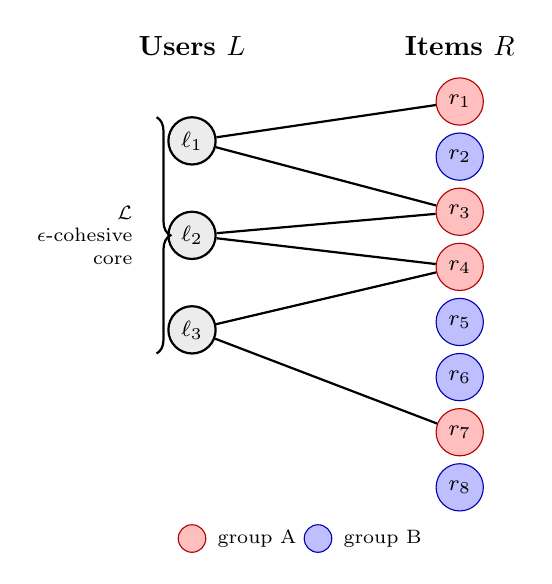
\begin{tikzpicture}[
    >=Stealth,
    user/.style={circle, draw=black, thick, fill=gray!15,
        minimum size=6mm, inner sep=0pt},
    red item/.style={circle, draw=red!70!black, fill=red!25,
        minimum size=6mm, inner sep=0pt},
    blue item/.style={circle, draw=blue!70!black, fill=blue!25,
        minimum size=6mm, inner sep=0pt},
    coreedge/.style={black, thick},
    every node/.style={font=\footnotesize}
]

% Column headings
\node[font=\bfseries] at (0,5.6) {Users $L$};
\node[font=\bfseries] at (3.4,5.6) {Items $R$};

% Left vertices
\node[user] (u1) at (0,4.4) {$\ell_1$};
\node[user] (u2) at (0,3.2) {$\ell_2$};
\node[user] (u3) at (0,2.0) {$\ell_3$};

% Right vertices
\node[red item]  (v1) at (3.4,4.9) {$r_1$};
\node[blue item] (v2) at (3.4,4.2) {$r_2$};
\node[red item]  (v3) at (3.4,3.5) {$r_3$};
\node[red item]  (v4) at (3.4,2.8) {$r_4$};
\node[blue item] (v5) at (3.4,2.1) {$r_5$};
\node[blue item] (v6) at (3.4,1.4) {$r_6$};
\node[red item]  (v7) at (3.4,0.7) {$r_7$};
\node[blue item] (v8) at (3.4,0.0) {$r_8$};

% Edges: theta = 2, with each user connected to red items
\draw[coreedge] (u1)--(v1);
\draw[coreedge] (u1)--(v3);
\draw[coreedge] (u2)--(v3);
\draw[coreedge] (u2)--(v4);
\draw[coreedge] (u3)--(v4);
\draw[coreedge] (u3)--(v7);

% Core brace
\draw[decorate, decoration={brace, amplitude=5pt}, thick]
    (-0.45,4.7) -- (-0.45,1.7)
    node[midway, left=5pt, align=right, font=\scriptsize]
    {$\mathcal{L}$\\$\epsilon$-cohesive\\core};

% Legend
\node[red item, minimum size=3.5mm] at (0,-0.65) {};
\node[anchor=west, font=\scriptsize] at (0.2,-0.65)
    {group A};
\node[blue item, minimum size=3.5mm] at (1.6,-0.65) {};
\node[anchor=west, font=\scriptsize] at (1.8,-0.65)
    {group B};

\end{tikzpicture}
\caption{Example with $\theta=2$. Same-colored items are within
$\epsilon$ of each other, while differently colored items are not.
For $\mathcal{L}=\{\ell_1,\ell_2,\ell_3\}$,
$N(\mathcal{L})=\{r_1,r_3,r_4,r_7\}$ contains only red items,
so $M_{\mathcal{L}}<\epsilon$. Every user has at least $\theta$
neighbors, but the users do not share a common neighborhood:
no biclique larger than $2\times1$ exists on these users.
Of the 12 possible edges between $\mathcal{L}$ and
$N(\mathcal{L})$, only 6 exist. Thus, the example illustrates
how the model can capture users connected to similar, but not
identical, items.}
\label{fig:epsilon-cohesive-core}
\end{figure}

\section{Proof of NP-hardness}

I was not able to fully prove that this graph formulation is NP-hard. However, here is my intuition for a reduction:

Let $G = (V, E_G)$. Construct a bipartite graph $B = (L, R, E_B)$ where $L = V$, $R = V$, and edges exist between every $(\ell, r) \mathrel{\text{s.t.}} \ell = r$. In other words, the bipartite graph is entirely a matching. This reduction takes $\mathcal{O}(|V|)$ because it must create $2|V|$ vertices and $|V|$ edges, so it is therefore a polynomial-time reduction.

Fix $\epsilon = 2$, $\theta = 1$, and

\begin{equation}
d(r_1, r_2) = 
\begin{cases}
    0 & \text{if } r_1 = r_2 \\
    1 & \text{if } (r_1, r_2) \in E_G \mathrel{\text{or}} r_1 = r_2 \\
    3 & \text{otherwise}
\end{cases}
\end{equation}

Each vertex $\ell \in L$ has exactly one neighbor (itself), so with $\theta = 1$, every subset of $L$ satisfies the minimum degree constraint.

Because $d \in \{1, 3\}$ and $\epsilon = 2$, two vertices meet the similarity constraint iff they have an edge between them. Therefore, if $M < \epsilon$, then all vertices in $N(\mathcal{L})$ must have an edge between every other vertex, and therefore they must form a clique. Finding the maximum number of vertices $\ell \in \mathcal{L}$ is equivalent to finding the maximum number of clique vertices $r \in V$, because the bipartite graph has a one-to-one matching. Therefore, for a given $\ell \in \mathcal{L}$, $N(\ell) = \{\ell\}$.

Because two vertices are considered similar iff they have an edge between them, finding a group of vertices that are all similar to each other is equivalent to finding a clique. Therefore, finding the maximum $\epsilon$-cohesive core is equivalent to finding the maximum clique in $G$.

I believe this reduction from Max CLIQUE establishes NP-hardness of the optimization variant of this problem. I would appreciate feedback on whether this seems intuitively valid as I try to formalize this proof.

\section{Literature Review}

To my knowledge, this exact formulation has not been studied.

It is most similar to Yao et al. \cite{yao2022identifying}. They proposed a biclique in which vertices on the same side are similar. They define two vertices as being similar if the Jaccard similarity of their neighbors is $\geq$ some threshold $\epsilon$. However, Yao et al. do not generalize this similarity to some arbitrary distance function, and they require the model to be a biclique.

The formulation may also be thought of as a mapping of the geo-social group (GSG) proposed by Li \& Zlatanova \cite{li2021significant}. This problem relates to a graph where each node has an associated 2D coordinate pair. The GSG is the largest group of nodes whose coordinates all fall within an enclosing circle of radius $\leq \gamma$ for some threshold $\gamma$.

\section{Future Idea}

Set an overlap parameter $I$ such that $|\bigcap_{\ell \in \mathcal{L}}N(\ell)| \geq I$. For example, if $I = 1$, everyone has to have bought at least 1 exactly identical product.

\end{document}